\documentclass[12pt,a4paper]{article}

\usepackage[margin=2cm]{geometry}
\usepackage[T1]{fontenc}
\usepackage[utf8]{inputenc}
\usepackage{graphicx}
\usepackage{parskip}
\usepackage{titlesec}
\usepackage{lmodern}
\usepackage{hyperref}
\usepackage{xcolor}
\usepackage{booktabs}
\usepackage{tabularx}
\usepackage{ragged2e}

\hypersetup{colorlinks=true, linkcolor=black, urlcolor=black}
\titleformat{\section}{\large\bfseries}{}{0em}{}[\titlerule]

\begin{document}

% ─── Title block ─────────────────────────────────────────────────────────────
\begin{center}
    {\LARGE\bfseries Spotly --- Data Model}\\[0.4em]
    {\large UML Class Diagram}\\[0.8em]
    \begin{tabular}{ll}
        \textbf{Course:}      & ISS296 --- Spring 2026 \\
        \textbf{Instructor:}  & Mr. Amine Ben Hassouna \\
        \textbf{Team:}        & Cyrine Krichen, Eya Sassi, \\
                              & Lina Khemiri, Youssef Ben Jemaa \\
    \end{tabular}
\end{center}

\vspace{0.6em}
\hrule
\vspace{0.8em}

% ─── Introduction ────────────────────────────────────────────────────────────
\section{Overview}

The Spotly data model consists of \textbf{eight entity classes} persisted in
the browser's local storage. Each class has a dedicated storage key and
follows a reactive CRUD pattern. There is no backend: the application is
entirely frontend-driven and data is shared across browser tabs via the
Web Storage \texttt{storage} event.

The diagram uses standard UML class notation. Relationships show the
foreign-key field used for association (e.g.\ \texttt{venueId},
\texttt{userId}). Composition arrows (\emph{filled diamond}) indicate that
child objects have no independent existence outside their parent.

\vspace{0.5em}
\textbf{Persistence keys:}

\vspace{0.3em}
{\small
\begin{tabularx}{\linewidth}{llX}
    \toprule
    Class & Storage Key & Notes \\
    \midrule
    User            & \texttt{spotly\_users}             & Email used as natural key \\
    Venue           & \texttt{spotly\_venues}            & Linked to User via \texttt{adminEmail} \\
    Environment     & \texttt{spotly\_environments}      & Contains embedded \texttt{FloorElement} array \\
    MenuItem        & \texttt{spotly\_menu\_items}       & Scoped to venue; optionally to specific environments \\
    Reservation     & \texttt{spotly\_reservations}      & \RaggedRight Status: REQUESTED $|$ APPROVED $|$ REJECTED $|$ CANCELLED $|$ CHECKED\_IN $|$ COMPLETED $|$ NO\_SHOW \\
    Review          & \texttt{spotly\_reviews}           & Status: VISIBLE $|$ HIDDEN \\
    VenueStaff      & \texttt{spotly\_venue\_staff}      & Junction table linking User to Venue as staff \\
    WaiterCall      & \texttt{spotly\_waiter\_calls}     & Status: pending $|$ acknowledged \\
    \bottomrule
\end{tabularx}
}

% ─── Diagram ─────────────────────────────────────────────────────────────────
\section{Class Diagram}

\vspace{0.3em}
\begin{center}
    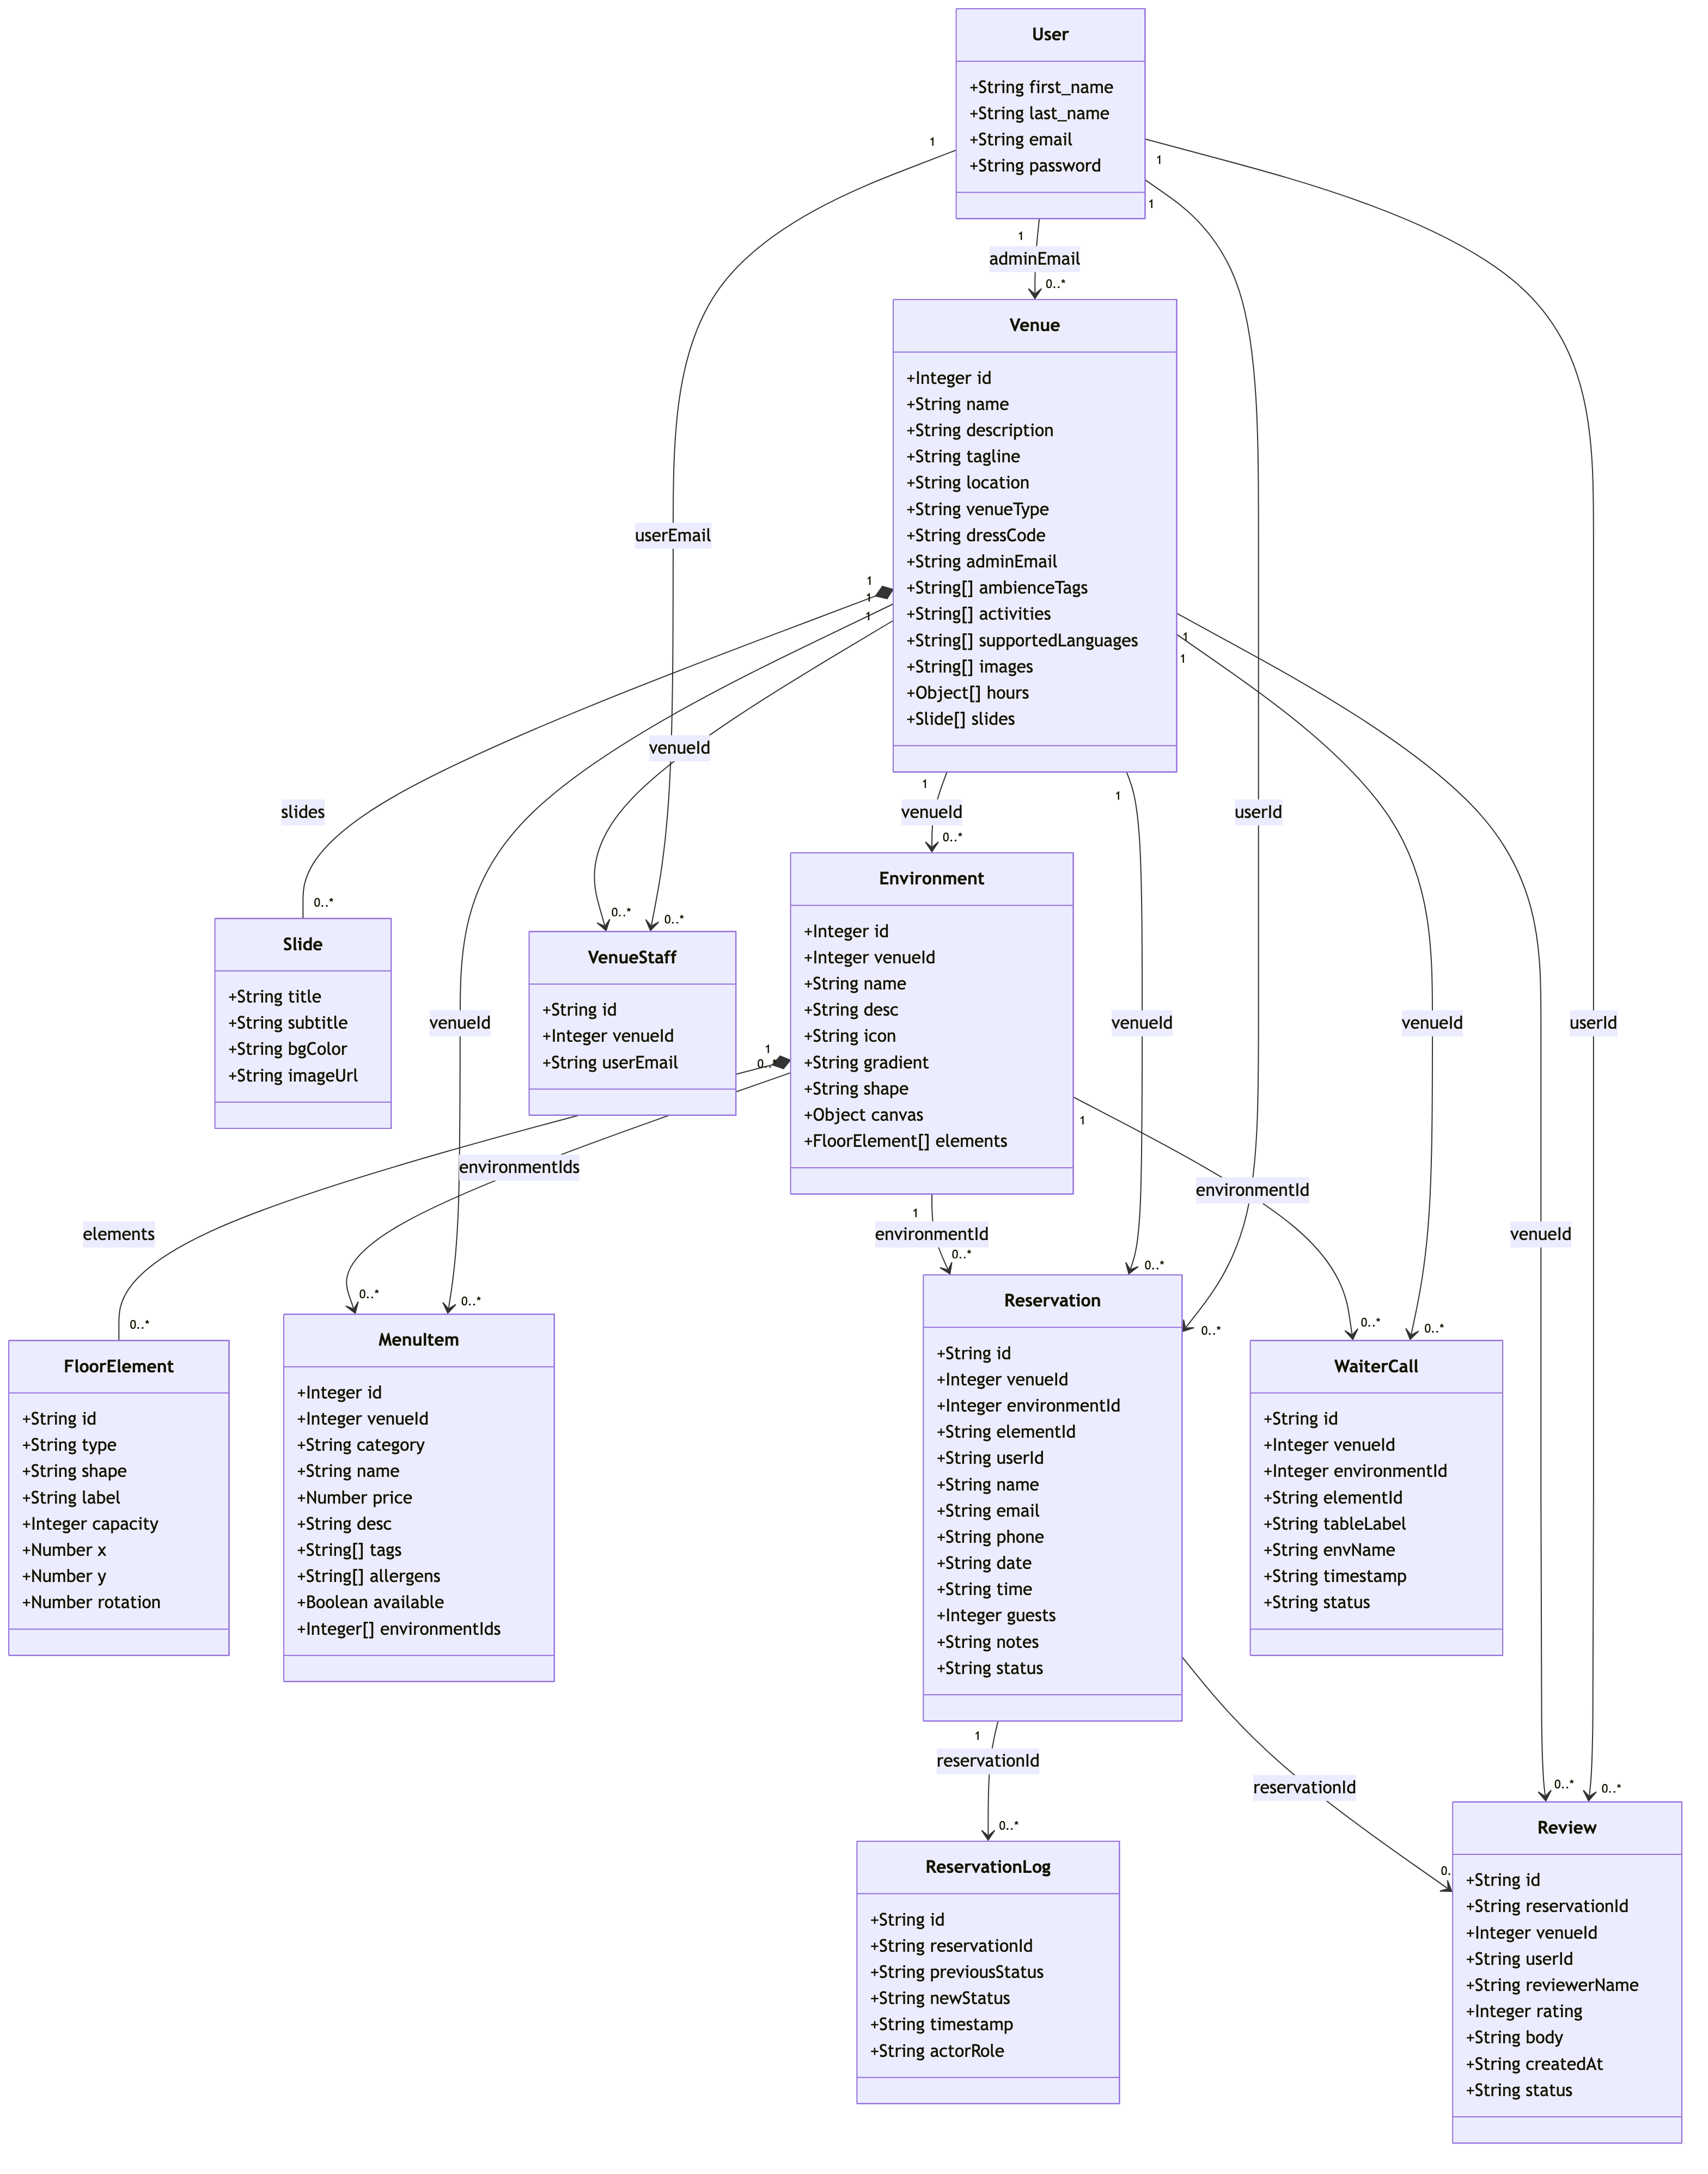
\includegraphics[width=\linewidth, keepaspectratio]{class.png}
\end{center}

\end{document}
